\documentclass[12pt,xcolor=table,aspectratio=169]{beamer}
\usetheme{Frankfurt}
\usecolortheme{rose}
\usepackage{amsthm}
\usepackage{amsmath}
\usepackage{bbm}
\usepackage{amsfonts}
\usepackage{amssymb}
\usepackage{graphicx}
\usepackage{hyperref}
\usepackage[flushleft]{threeparttable}
\usepackage{tabularx}
\usepackage{booktabs}
\usepackage{siunitx}
\usepackage{tikz}
\usetikzlibrary{decorations.pathreplacing,angles,quotes}
%\usepackage{enumitem}% http://ctan.org/pkg/enumitem

%set up course and number

\newcommand{\ClassName}{TBD}
\newcommand{\ClassNumber}{TBD}
\newcommand{\Topic}{TBD}

% Some optional colors. Change or add as you see fit.
%---------------------------------------------------
 \definecolor{ualbertagreen}{HTML}{007C41}
\definecolor{ualbertagold}{HTML}{FFDB05}

\definecolor{calloutgrey}{HTML}{D9D9D9}


%set fonts
\setbeamerfont{subtitle}{size=\large,shape=\scshape,series=\bfseries}
\setbeamerfont{title}{size=\Large,shape=\scshape,series=\bfseries}
\setbeamerfont{author}{size=\large}
\setbeamerfont{date}{size=\large}
\setbeamerfont{caption}{size=\scriptsize}


% Some optional color adjustments to Beamer. Change as you see fit.
%------------------------------------------------------------------
\setbeamercolor{frametitle}{fg=ualbertagreen,bg=white}
\setbeamercolor{title}{fg=ualbertagreen,bg=white}
\setbeamercolor{author}{fg=ualbertagreen,bg=white}
\setbeamercolor{date}{fg=ualbertagreen,bg=white}
\setbeamercolor{local structure}{fg=ualbertagreen}
\setbeamercolor{section in toc}{fg=ualbertagreen,bg=white}
% \setbeamercolor{subsection in toc}{fg=ualbertagreen,bg=white}
\setbeamercolor{footline}{fg=ualbertagreen!50, bg=white}

% definition boxes
\setbeamercolor{block title}{bg=ualbertagreen,fg=white}
\setbeamercolor{block body}{parent=normal text,use=block title,bg=calloutgrey}
%\setbeamercolor{block body}{parent=normal text,use=block title,bg=block title.bg!30!bg}


\setbeamercolor{upper separation line head}{bg=ualbertagreen}
\setbeamercolor{lower separation line head}{bg=ualbertagold}
\setbeamercolor{middle separation line head}{bg=ualbertagold}
\setbeamercolor{frametitle}{fg=ualbertagreen,bg=white}



\setbeamercolor{section in head/foot}{bg=white,fg=ualbertagreen}
\setbeamercolor{author in head/foot}{bg=white,fg=ualbertagreen}
\setbeamercolor{date in head/foot}{bg=white,,fg=ualbertagreen}
\setbeamercolor{title in head/foot}{bg=white,fg=ualbertagreen}

\setbeamercolor{headline}{bg=white,fg=ualbertagreen}




\setbeamercolor*{middle separation line head}{bg=ualbertagreen}
\setbeamercolor*{alerted text}{fg=black}
\setbeamerfont{alerted text}{series=\bfseries}
\setbeamercolor*{example text}{fg=black}
\setbeamercolor*{structure}{fg=black}


\let\Tiny=\tiny



\logo{
   %\ifnum\insertpagenumber>1
   \tikz [remember picture,overlay]
    \node[yshift=.3cm,xshift=1.5cm] at (current page.south west)
        %or: (current page.center)
        {
\includegraphics[width=1in]{../images/UA-ASB-COLOUR.png}};
    %\fi
%
\includegraphics[height=0.8cm]{../images/UA-ASB-COLOUR.png}\vspace{220pt}
}


\setbeamertemplate{title page}{%
  \vbox{}
    \vspace{.5cm}% NEW
  \begingroup
    \centering
    \begin{beamercolorbox}[sep=8pt,center]{title}
      \usebeamerfont{title}\ClassNumber: \ClassName\par%
      \usebeamerfont{title}\inserttitle\par%
     \ifx\insertsubtitle\@empty%
      \else%
        \vskip0.05em%
        {\usebeamerfont{subtitle}\usebeamercolor[fg]{subtitle}\insertsubtitle\par}%
      \fi%
    \end{beamercolorbox}%
    \begin{beamercolorbox}[sep=8pt,center]{author}
      \usebeamerfont{author}\insertauthor
    \end{beamercolorbox}
    \begin{beamercolorbox}[sep=8pt,center]{institute}
      \usebeamerfont{institute}\insertinstitute
    \end{beamercolorbox}

    \vspace{0.5cm}% NEW
    \begin{beamercolorbox}[sep=8pt,center]{date}
      \usebeamerfont{date}\insertdate
    \end{beamercolorbox}\vskip0.05em

      \endgroup
  %\vfill
}


\setbeamertemplate{frametitle}{%
    \insertframetitle\par\vskip-10pt
}



\renewcommand{\ClassName}{Business Economics, Organization and Management}
\renewcommand{\ClassNumber}{BUEC 311}

\setbeamertemplate{headline}{%
\leavevmode%
 \hbox{%
    \begin{beamercolorbox}[wd=\paperwidth,ht=5ex,dp=0ex]{white}%
    \usebeamerfont{headline}\hskip6pt\ClassNumber: \inserttitle\par%
    \insertsectionnavigationhorizontal{\paperwidth}{}{\hskip0pt plus1filll}
    \end{beamercolorbox}%
  }
}

\defbeamertemplate*{footline}{my footline}{%
    \ifnum\insertpagenumber=1
        \Tiny{%
            \hfill%
		\vspace*{1pt}%
            %\insertframenumber/\inserttotalframenumber \hspace*{0.1cm}%
            \newline%
            \color{ualbertagold}{\rule{\paperwidth}{0.4mm}}\newline%
            \color{ualbertagold}{\rule{\paperwidth}{.4mm}}%
        }
  \else%
        \Tiny{%
            \hspace{.66\paperwidth}
            %\vspace{25pt}
            \insertframenumber/\inserttotalframenumber
            \newline%
            \color{ualbertagold}{\rule{\paperwidth}{0.4mm}}\newline%
            \color{ualbertagold}{\rule{\paperwidth}{.4mm}}%
        }%
    \fi%
}


\newenvironment{itemize*}%
  {\begin{itemize}%
    \setlength{\itemsep}{0pt}%
    \setlength{\parskip}{0pt}}%
  {\end{itemize}}


\title{
	Producer Behaviour, Part 3
}

\date{Professor Andrew Leach}

\begin{document}

\section{Outline}


\frame{
	\titlepage
}

\frame{
	\frametitle{Outline}
	\begin{enumerate}
	\item The Ownership and Governance of Firms
	\item[]
	\item Profit Maximization
	\item[]
	\item Owners' vs. Managers' Objectives
	\item[]
	\item The Make or Buy Decision
	\item[]
	\item Market Structure
	\end{enumerate}
}

\frame{
	\frametitle{Outline}
	\begin{enumerate}
	\item \alert{The Ownership and Governance of Firms}
	\item[]
	\item Profit Maximization
	\item[]
	\item Owners' vs. Managers' Objectives
	\item[]
	\item The Make or Buy Decision
	\item[]
	\item Market Structure
	\end{enumerate}
}

\section{Ownership and Governance}

\frame{
	\frametitle{Economic sectors}
	\begin{itemize}
	\item Firms operate in one of three sectors:
		\begin{enumerate}
		\item The \underline{Private Sector}: Firms that are owned by individuals or non government entities and whose owners may earn a profit.
			\begin{itemize}
			\item E.g. Apple, Heinz, Toyota.
			\item In most countries, the private sector accounts for the largest fraction of economic output.
			\end{itemize}
				\item The \underline{Public Sector}: Firms and other organizations that are owned by governments or government agencies; also called \textit{state-owned enterprises}.
			\begin{itemize}
			\item E.g. Armed forces, education, health care, Canada Post, Via Rail.
			\item The public sector can be large or small; typically between 10-20\% of economic output.
			\end{itemize}
			\item The \underline{Nonprofit Sector}: Organizations that are neither government owned, nor intended to earn a profit, but typically pursue social or public interest objectives.
			\begin{itemize}
			\item E.g. Greenpeace, Alcoholics Anonymous, the Salvation Army.
			\end{itemize}
		\end{enumerate}
	\end{itemize}
}

\frame{
	\frametitle{Ownership Structures}
	\begin{itemize}
	\item There are three main ownership structures for firms in the private sector:
		\begin{enumerate}
		\item \underline{Sole proprietorships} are firms owned and controlled by a single individual.
		\item[]
		\item \underline{Partnerships} are businesses jointly owned and controlled by two or more individuals operating under a partnership agreement.
		\item[]
		\item \underline{Corporations} are firms owned by \underline{shareholders}, who own the firm's \underline{shares or stocks}.
			\begin{itemize}
			\item A share is a unit of ownership of the firm. A shareholder's ownership is proportional to the number of shares they hold.
			\item Shareholders typically elect a board of directors to represent them. The board of directors hires managers to run the firm's operations.
			\item The legal name of a corporation often includes the term ``Incorporated'' (Inc.) or ``Limited'' (Ltd.) to indicate its corporate status.
			\end{itemize}
		\end{enumerate}
	\end{itemize}
}

\frame{
	\frametitle{Public vs Private}
	\begin{itemize}
	\item Shares of \textit{public corporations} can be bought and sold by the general public.
		\begin{itemize}
		\item Shares may be available on an organized stock exchange, such as the New York Stock Exchange, the NASDAQ, the Tokyo Stock Exchange, the Toronto Stock Exchange, or the London Stock Exchange.
		\end{itemize}
	\item Shares of \textit{closely held corporations} are not available for purchase or sale on an organized exchange.
		\begin{itemize}
		\item Typically its stock is owned by a small group of individuals (\underline{private equity}).
		\end{itemize}
	\item To transition from privately held to publicly traded status, a closely held firm will typically make an initial public offering (IPO) of its shares on an organized stock exchange.
		\begin{itemize}
		\item Why go public?
		\end{itemize}
	
	\item Firms can also transition from being publicly traded to being closely held.
		\begin{itemize}
		\item E.g. Toys-R-Us, Burger King.
		\end{itemize}
	\end{itemize}
}

\frame{
	\frametitle{Corporations}
	\begin{itemize}
	\item Owners of a corporation are not personally liable for the firm's debts.
		\begin{itemize}
		\item They have \underline{limited liability}: personal assets cannot be taken to pay a corporation's debts, even if it goes into bankruptcy.
		\end{itemize}
	\item[]
	\item Historically, owners of sole proprietorships and partnerships were fully liable, individually and collectively for any debts of the firm.
		\begin{itemize}
		\item Now owners can form a limited liability company (LLC).
		\item The precise regulations governing LLCs varies from country to country.
		\end{itemize}
	\end{itemize}
}

\frame{
	\frametitle{Limited Liability}
	\begin{itemize}
	\item Key benefit of limiting liability for firm owners: firms can grow larger.
	\item[]
	\item In the U.S., most large firms are corporations.
		\begin{itemize}
		\item According to the 2015 ProQuest Statistical Abstract of the U.S., U.S. corporations are only 18\% of all non-farm firms, but make 81\% of sales revenue and 58\% of net income. Non-farm sole proprietorships are 72\% of firms, but make only 4\% of sales revenue and 15\% of net income.
		\item Less than 1\% of U.S. corporations earn over \$50 million, but they account for 77\% of total revenue.
		\end{itemize}
	\item[]
	\item The available data suggests the pattern in Canada is similar.
	\end{itemize}
}

\frame{
	\frametitle{Distribution of Firms}
\vspace{-.1cm}	
\begin{figure}
	\centering
	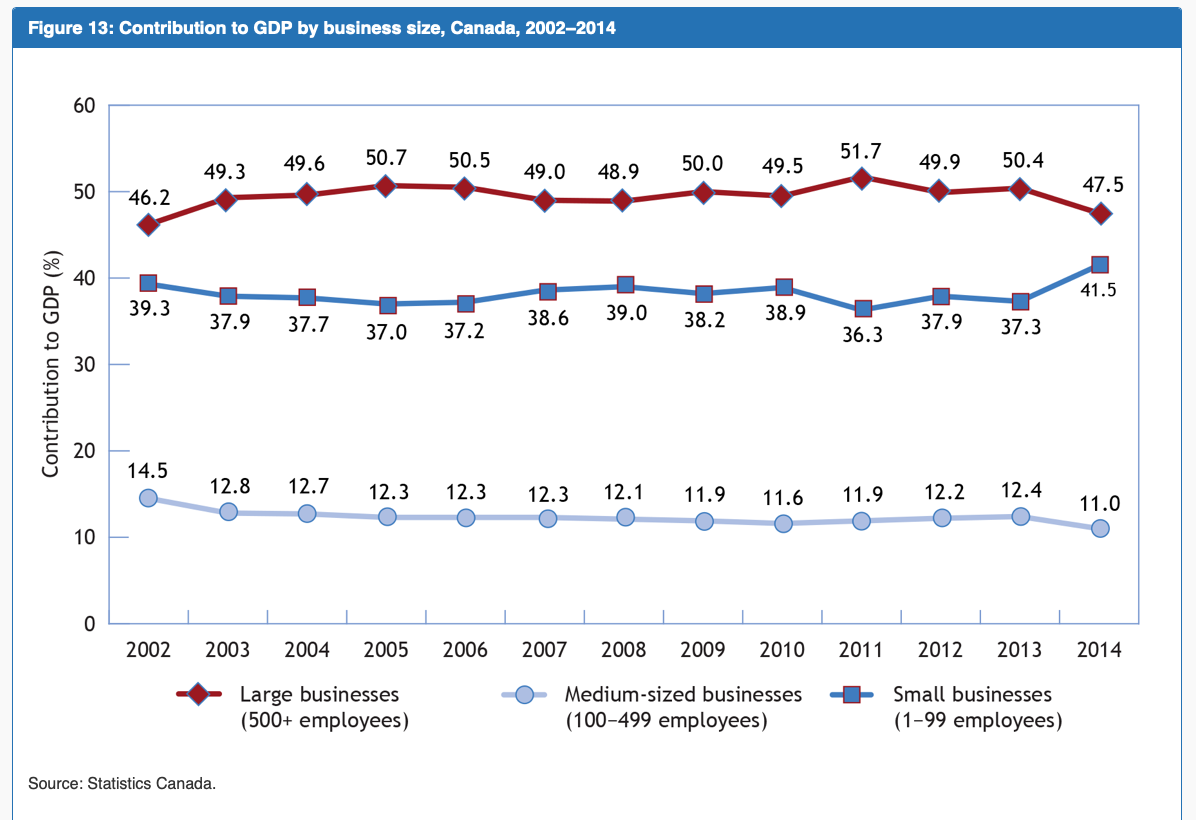
\includegraphics[scale=.225]{../images/gdp.png}
	\end{figure}
	}

\frame{
	\frametitle{Distribution of Firms}
	\begin{figure}
	\centering
	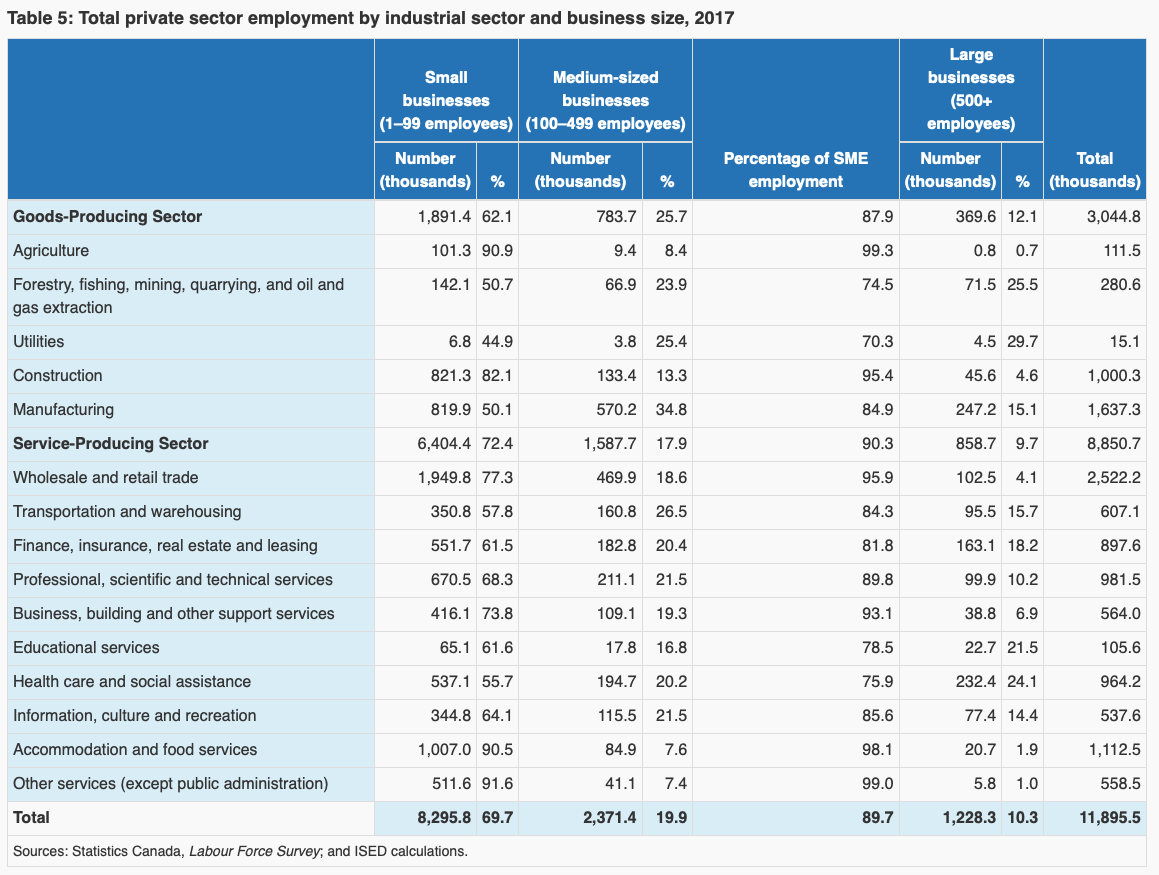
\includegraphics[scale=.225]{../images/employment_by_industry.png}
	\end{figure}
	}

\frame{
	\frametitle{Distribution of Firms}
	\begin{figure}
	\centering
	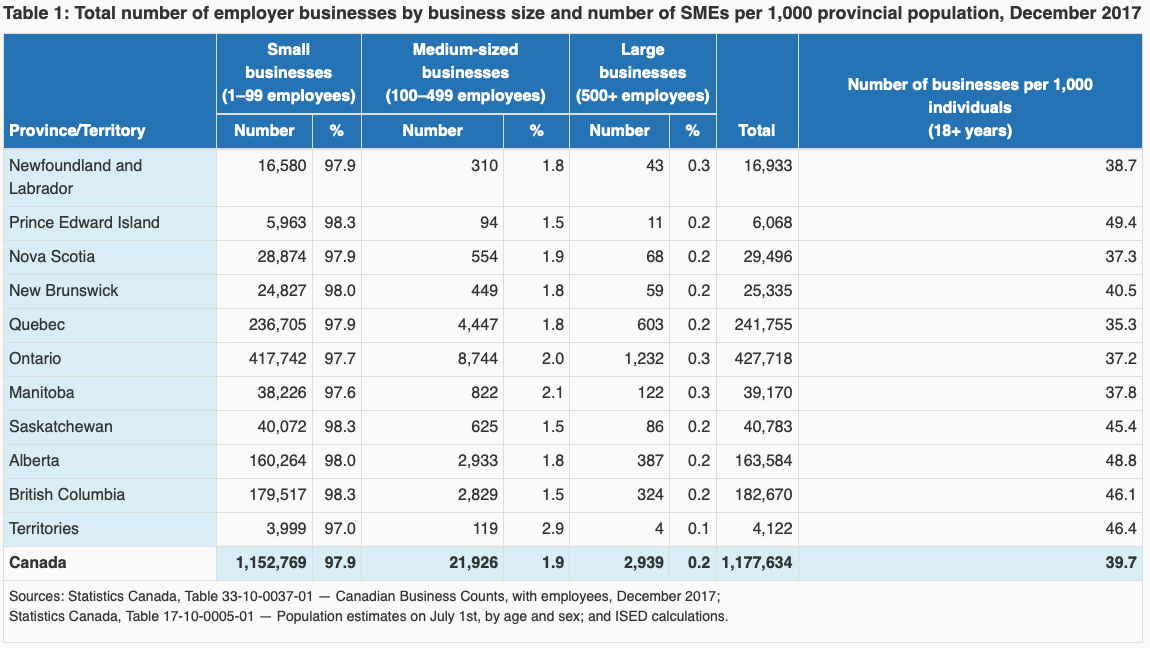
\includegraphics[scale=.225]{../images/employment_by_province.png}
	\end{figure}
	}

\frame{
	\frametitle{Governance}
	\begin{itemize}
	\item In a small private sector firm with a single owner/manager, the governance of a firm is straightforward.
		\begin{itemize}
		\item The owner/manager makes the important decisions for the firm.
		\end{itemize}
	\item In publicly traded companies, the shareholders own the corporation. However, most play no meaningful role in day-to-day decision making or long range planning.
		\begin{itemize}
	\item Shareholders elect a board of directors and delegate many of their ownership rights to them.
	\item The board of a large publicly traded corporation normally includes outside directors and inside directors, such as the chief executive officer (CEO) of the corporation, and other senior executives.
	\end{itemize}
	
	\end{itemize}
}

\section{Profit Maximization}

\frame{
	\frametitle{Outline}
	\begin{enumerate}
	\item The Ownership and Governance of Firms
	\item[]
	\item \alert{Profit Maximization}
	\item[]
	\item Owners' vs. Managers' Objectives
	\item[]
	\item The Make or Buy Decision
	\item[]
	\item Market Structure
	\end{enumerate}
}



\frame{
	\frametitle{Profit Maximization}
	\begin{itemize}
	\item Main goal of most firms in the private sector: \textit{maximize profit}
	\item[]
	\item Profit ($\pi$) is the difference between a firm's revenues ($R$) and costs ($C$):
		\begin{align*}
		\pi = R - C
		\end{align*}
	\item If profit is negative $(\pi<0)$, the firm makes a loss.
	\end{itemize}
}	

\frame{
	\frametitle{Profit Maximization and Opportunity Costs}
	\begin{itemize}
	\item \underline{Firm profit}:
		\begin{align*}
		\pi = R - C
		\end{align*}
	\item \underline{Revenue} is price times quantity ($R= p \times q$), although may also include non-market valued items.
	\item[]
	\item \underline{Cost} is measured using \textit{opportunity cost}, the value of the best alternative use of any input the firm employs.
		\begin{itemize}
		\item Recall: the full opportunity cost of inputs (or value of output) used may exceed the explicit or out-of-pocket costs (or into-pocket revenues) recorded in financial accounting statements.
		\end{itemize}
	\end{itemize}
}

\frame{
	\frametitle{Profit Maximization and output}
	\begin{itemize}
	\item Because revenue and cost both vary with output, $q$, the firm's profit also varies with output:
		\begin{align*}
		\pi (q) = R(q) - C(q)
		\end{align*}
	\item Key question: What level of output, $q$, should the firm choose?
	\end{itemize}
}

\frame{
	\frametitle{Profit Functions}
	\begin{itemize}
	\item If the firm knows how profit changes with $q$, it can choose the $q$ that yields the highest level of profit. That is, it can choose the \textit{profit maximizing} level of $q$.
	\item[]
	\item This is the same as the firm picking the highest point on its \textit{profit curve}.
	\end{itemize}
}

\frame{
	\frametitle{Profit Maximization}
	\begin{figure}[t!]
	\center
	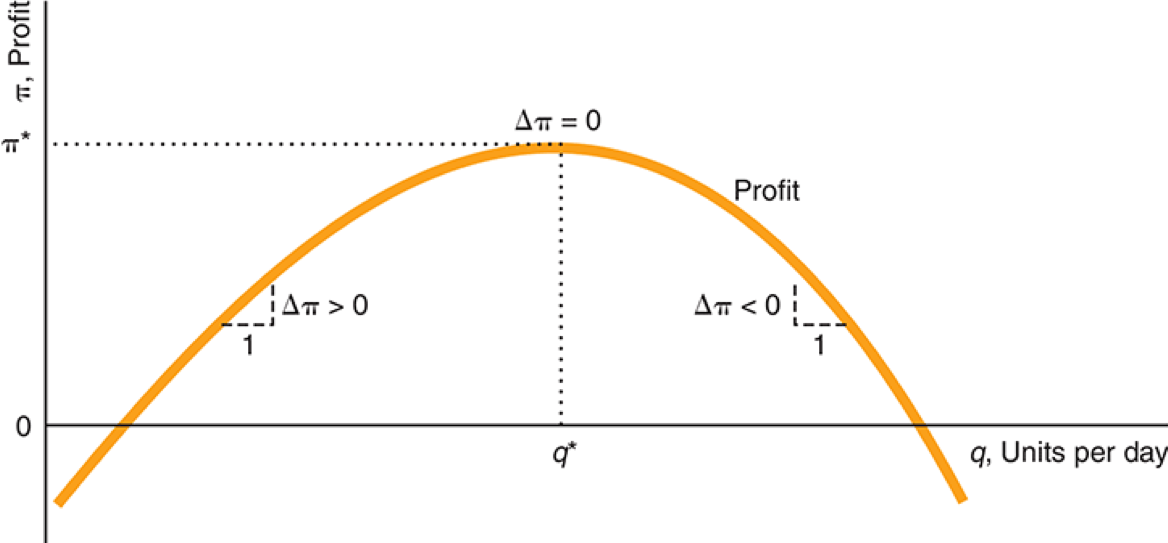
\includegraphics[scale=0.5]{../images/pi_max.png}
	\end{figure}
}

\frame{
	\frametitle{Profit Maximization}
	\begin{itemize}
	\item Unfortunately, the shape of the profit curve is not always known.
	\item[]
	\item In this case, the firm can find the profit maximizing level of output though experimentation:
		\begin{itemize}
		\item If the firm increases output by a small amount, and profit increases, it should keep increasing output until doing so does not increase profit any further.
		\item If the firm increases output by a small amount, and profit decreases, it should decrease output until doing so does not decrease profit any further.
		\end{itemize}
	\item[]
	\item This experimentation yields the peak of the profit curve.
		\begin{itemize}
		\item Why? Think about the end points.
		\end{itemize}
	\end{itemize}
}

\frame{
	\frametitle{Profit Maximization}
	\begin{figure}[t!]
	\center
	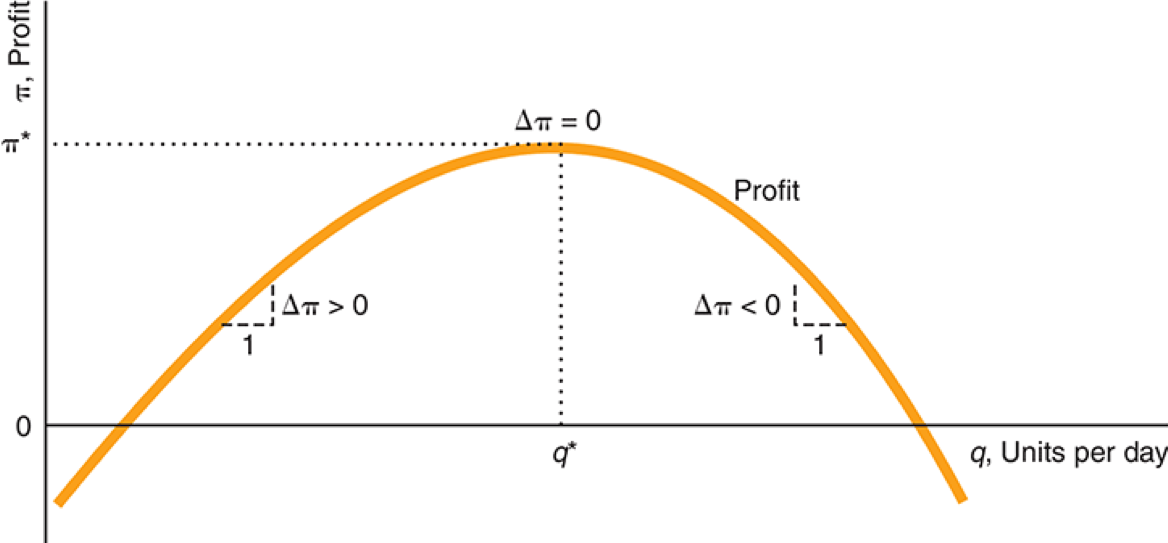
\includegraphics[scale=0.5]{../images/pi_max.png}
	\end{figure}
}

\frame{
	\frametitle{Profit Maximization at the Margin}
	\begin{itemize}
	\item We can also determine the peak of the profit curve from changes in marginal revenue ($MR(q)$) and marginal costs ($MC(q)$).
		\begin{align*}
		\text{Marginal Profit}(q) = MR(q) - MC(q)
		\end{align*}
	\item Marginal profit increasing if $MR(q)>MC(q)$.
	\item[]
	\item Marginal profit decreasing if $MR(q)<MC(q)$.
	\item[]
	\item Profit is maximized when $MR(q) = MC(q)$.
	\end{itemize}
}

\frame{
	\frametitle{Profit Maximization and Losses}
	\begin{itemize}
	\item It is possible that the firm may make a loss even at its profit maximizing level of output.
	\item[]
	\item Key question:
		\begin{itemize}
		\item Should the firm continue to operate if its profit is negative?
		\end{itemize}
	\end{itemize}
}

\frame{
	\frametitle{Firm Exit Decisions}
	\begin{itemize}
	\item In general, a firm should shut down only if it can reduce its loss by doing so.
		\begin{itemize}
		\item This applies in both the short and long run alike.
		\end{itemize}
	\item[]
	\item The firm should shut down only if its revenue is less than its avoidable cost.
		\begin{itemize}
		\item In the short run, variable costs are \underline{avoidable}, but most fixed costs are \underline{unavoidable} (sunk costs).
		\item In the long run, all costs are \underline{avoidable}.
		\end{itemize}
	\end{itemize}
}		

\frame{
	\frametitle{Dynamic or Long-term Profit Maximization}
	\begin{itemize}
	\item Of course, firms need not only focus on the current period.
		\begin{itemize}
		\item Normally, firms are interested in maximizing profit over many periods.
		\end{itemize}
	\item[]
	\item Because money today is worth more than money in the future, a stream of future profits is valued using its present value:
		\begin{align*}
		PV = \frac{FV}{(1+i)^{t}}
		\end{align*}
		where $PV$ is the present value, $FV$ is the future value, $i$ is the interest rate, and $t$ is the number of years.
	\end{itemize}
}

\frame{
	\frametitle{Profit Maximization and Share Prices}
	\begin{itemize}
	\item Should manager focus on maximizing profit or share price?
	\item[]
	\item Depends on how knowledgeable investors are.
		\begin{itemize}
		\item If investors are well informed, stock price reflect current and future profits of the firm.
		\item If investors are not well informed, stock price may not reflect profits.
		\end{itemize}
	\end{itemize}
}

\frame{
	\frametitle{Outline}
	\begin{enumerate}
	\item The Ownership and Governance of Firms
	\item[]
	\item Profit Maximization
	\item[]
	\item \alert{Owners' vs. Managers' Objectives}
	\item[]
	\item The Make or Buy Decision
	\item[]
	\item Market Structure
	\end{enumerate}
}

\section{Owners' vs. Managers' Objectives}

\frame{
	\frametitle{Owners' vs. Managers' Objectives}
	\begin{itemize}
	\item Key issue for firm owners:
		\begin{itemize}
		\item Getting managers to do what they want.
		\end{itemize}
	\item[]
	\item This is a form of a \textit{principal-agent} problem.
		\begin{itemize}
		\item Owner (principal) delegates tasks to managers (agents).
		\item Issue arises because principal and agent can have conflicting objectives:
			\begin{itemize}
			\item Owner wants to maximize profit.
			\item Managers want to maximize own income/perks.
			\end{itemize}
		\item If the owner and manager have different objectives, profit will not be maximized.
			\begin{itemize}
			\item This is an \textit{agency cost}.
			\end{itemize}
		\end{itemize}
	\end{itemize}
}

\frame{
	\frametitle{Owners' vs. Managers' Objectives}
	\begin{itemize}
	\item How can owners ensure managers do what they want?
	\end{itemize}
}

\frame{
	\frametitle{Owners' vs. Managers' Objectives}
	\begin{itemize}
	\item Two possible solutions:
		\begin{enumerate}
		\item \underline{Contingent rewards}.
			\begin{itemize}
			\item To align owner and manager objectives, many firms use contingent rewards: higher pay if the firm does well.
			\item e.g. Performance bonus, stock option.
			\end{itemize}
		\item[]
		\item \underline{Profit sharing}.
			\begin{itemize}
			\item Another option: pay the manager a share of the firm's profit.
			\item Requires that profit is easily observed, and both owner and manager want to maximize monetary payoffs.
			\end{itemize}
		\end{enumerate}
	\end{itemize}
}

\frame{
	\frametitle{Profit Sharing}
	\begin{figure}[t!]
	\center
	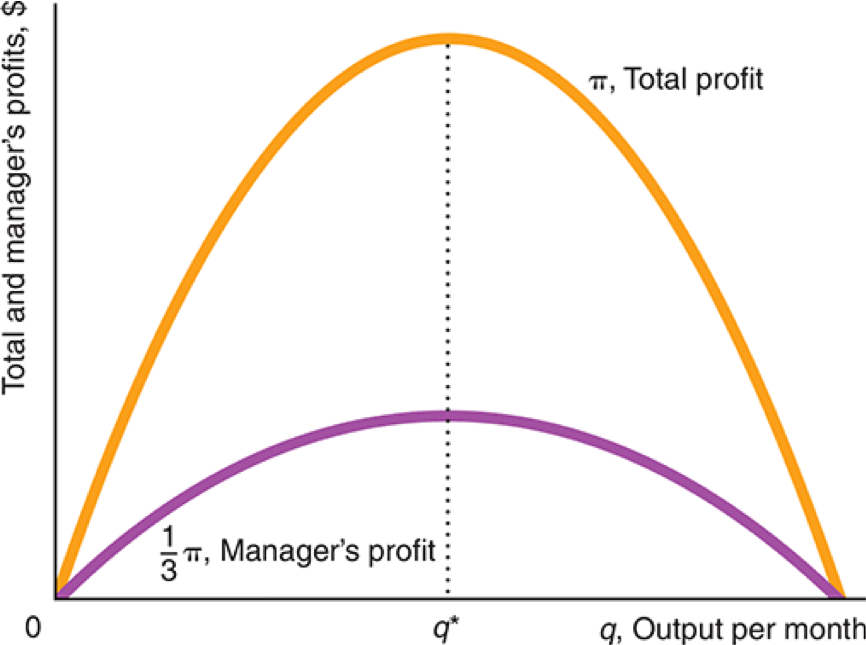
\includegraphics[scale=0.5]{../images/pi_share.png}
	\end{figure}
}

\frame{
	\frametitle{Profit Sharing}
	\begin{itemize}
	\item Profit sharing may not be possible in all cases.
		\begin{itemize}
		\item Profits may not be observable to all parties.
		\item Reported profit could be manipulated by owner or manager.
		\end{itemize}
	\item[]
	\item Common alternative to profit sharing: a revenue based objective.
		\begin{itemize}
		\item Manager either receives a fraction of firm revenue, or receives a payment tied to size of firm revenue.
		\item Would this work?
		\end{itemize}
	\end{itemize}
}

\frame{
	\frametitle{The Problem With Targeting Revenue}
	\begin{figure}[t!]
	\center
	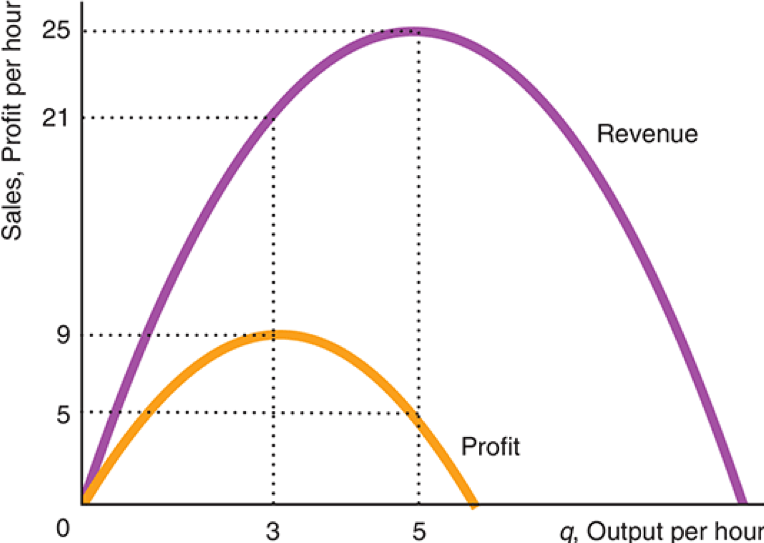
\includegraphics[scale=0.5]{../images/revenue_max.png}
	\end{figure}
}

\frame{
	\frametitle{The Manager's Objective}
	\begin{itemize}
	\item Owners also need to recognize that managers pursue objectives aside from maximizing their own income:
		\begin{enumerate}
		\item Minimizing effort.
			\begin{itemize}
			\item If compensation is not tied to performance, a manager may not try to maximize profit; may instead try to maximize own happiness.
			\item This can lead to \textit{satisficing} behaviour.
			\end{itemize}
		\item[]
		\item Maximizing perks.
			\begin{itemize}
			\item A manager may also try to maximize perks from job.
			\item Some perks save a manager's time, and increase productivity.
			\item Some perks have no tangible benefit to the firm; value of these perks should be deducted from the manager's salary.
			\end{itemize}
		\end{enumerate}
	\end{itemize}	
}

\frame{
	\frametitle{Social Objectives}
	\begin{itemize}
	\item Some firms pursue social objectives in addition to maximizing profit.
		\begin{itemize}
		\item These firms are engaged in \textit{Corporate Social Responsibility (CSR).}
		\end{itemize}
	\item[]
	\item The pursuit of CSR can be controversial.
		\begin{itemize}
		\item If management pursues social objectives, they may be reducing returns to shareholders.
        \item Key is to link the CSR to dynamic profit maximization.
		\end{itemize}
	\end{itemize}
}

\frame{
	\frametitle{Opposing Views on CSR}
	\begin{enumerate}
	\item Milton Friedman:
		\begin{itemize}
		\item The CSR of a firm is to increase its profits.
		\end{itemize}
	\item[]
	\item R. Edward Freeman:
		\begin{itemize}
		\item Firms have obligations to shareholders, workers, customers, and the community where firms reside and operate.
		\end{itemize}
	\end{enumerate}
}

\frame{
	\frametitle{Two Opposing Views on CSR}
	\begin{itemize}
	\item Who is right?
	\end{itemize}
}

\frame{
	\frametitle{Conflicting Objectives}
	\begin{itemize}
	\item If the owner and manager have conflicting objectives, the owner may try to monitor and control the manager's actions.
	\item[]
	\item This is straightforward if the owner and manager work side-by-side.
	\item[]
	\item Monitoring is difficult if:
		\begin{itemize}
		\item The owner cannot \underline{observe} the actions of the manager.
		\item Profits/payoffs from action is subject to \underline{uncertainty}.
		\end{itemize}
	\item[]
	\item Control is difficult if parties cannot write an \underline{enforceable contract}.
	\end{itemize}
}

\frame{
	\frametitle{Asymmetric Information}
	\begin{itemize}
	\item When a manager's actions are difficult to observe, owners need to rely on indirect monitoring.
	\item[]
	\item Indirect monitoring should be designed to reduce agency costs.
		\begin{itemize}
		\item \underline{Board and Managers}: Senior executives are restricted in their ability to carry out activities outside the firm (disclosure of conflict of interest).
		\item \underline{Shareholders and Board}: Rules may require firm to have outside directors; may also govern nature and frequency of elections.
			\begin{itemize}
			\item However, it can be difficult to specify/legally enforce what constitutes appropriate effort on the part of board members.
			\end{itemize}
		\item \underline{Say-on-Pay (SOP) rules}: Shareholders vote periodically on compensation going to senior executives.
			\begin{itemize}
			\item E.g. the Dodd-Frank Wall Street Reform, and the 2010 Consumer Protection Act.
			\item In Canada, SOP votes are not legally required, but voluntary use is increasing.
			\end{itemize}
		\end{itemize}
	\end{itemize}
}

\frame{
	\frametitle{Bad Outcomes}
	\begin{itemize}
	\item Markets can also discipline the behaviour of managers.
	\item[]
	\item \textit{Survivor principle}: In highly competitive markets, the only firms that survive are those that are run to maximize profit.
	\item[]
	\item \textit{Market for corporate control}: Outside investors buy enough shares to take over control of an under-performing publicly traded firm.
	\end{itemize}	
}

\frame{
	\frametitle{Poison Pills}
	\begin{itemize}
	\item In the United States, firms can defend against hostile takeovers with a \textit{shareholder rights plan}.
		\begin{itemize}
		\item Also known as a poison pill defence.
		\item Idea is to make a firm a less attractive takeover target by changing bylaws or charter.
		\end{itemize}
	\item[]
	\item Poison pills are restricted in many countries.
		\begin{itemize}
		\item In Canada, regulatory authorities often remove provisions deemed to be poison pills during takeover bids.
		\item Why would regulators do this?
		\end{itemize}
	\end{itemize}
}

\frame{
	\frametitle{Outline}
	\begin{enumerate}
	\item The Ownership and Governance of Firms
	\item[]
	\item Profit Maximization
	\item[]
	\item Owners' vs. Managers' Objectives
	\item[]
	\item \alert{The Make or Buy Decision}
	\item[]
	\item Market Structure
	\end{enumerate}
}

\section{Make or Buy?}

\frame{
	\frametitle{The Make or Buy Decision}
	\begin{itemize}
	\item Two key questions for management:
		\begin{enumerate}
		\item How large should the firm be in its primary market?
			\begin{itemize}
			\item This is the \textit{horizontal dimension} of the firm.
			\end{itemize}
		\item What stages of the production process should the firm participate in?
			\begin{itemize}
			\item This is the \textit{vertical dimension} of the firm.
			\end{itemize}
		\end{enumerate}
	\item[]
	\item The answer to 2. referred to as \textit{supply chain management}.
		\begin{itemize}
		\item Decision focuses on what sequential stages of production, marketing and distribution will be done in house, and what activities will be sourced from other firms.
		\end{itemize}
	\end{itemize}
}

\frame{
	\frametitle{The Make or Buy Decision}
	\begin{figure}
	\centering
	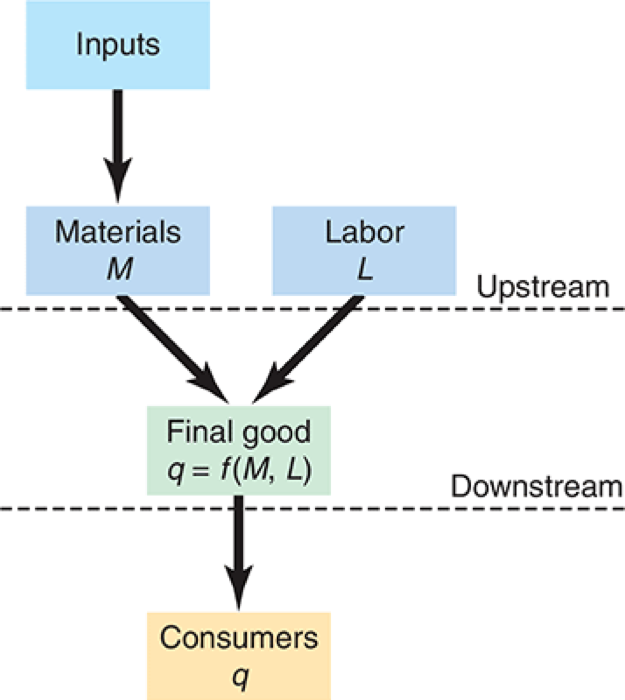
\includegraphics[scale=.5]{../images/vertical.png}
	\caption{A simple supply chain}
	\end{figure}
	}

\frame{
	\frametitle{The Make or Buy Decision}
	\begin{itemize}
	\item A firm that participates in more than one successive stage of production or distribution of goods and services is \underline{vertically integrated}.
	\item[]
	\item A firm may vertically integrate \underline{backward} and produce its own inputs, or \underline{forward} and buy its former customer.
	\item[]
	\item A firm can be partially vertically integrated.
		\begin{itemize}
		\item It can produce a good, but rely on another firm to market it.
		\item It may produce some inputs itself and buy others from the market.
		\end{itemize}
	\end{itemize}
}

\frame{
	\frametitle{Contracting}
	\begin{itemize}
	\item For many firms, it is possible to rely on \textit{spot markets} or \textit{cash markets} as a means to source inputs.
	\item[]
	\item Firms can also sign \textit{long-term contracts} to secure inputs at specified prices and quantities.
		\begin{itemize}
		\item Why contract instead of relying on the market?
		\end{itemize}
	\item[]
	\item Contracts can also be used to create \textit{vertical restraints} that lead to \textit{quasi-vertical integration}.
		\begin{itemize}
		\item E.g. Franchise and franchisee.
		\end{itemize}
	\item[]
	\item However, in practice, all firms are vertically integrated to some degree.
	\end{itemize}
}

\frame{
	\frametitle{Vertical Integration}
	\begin{itemize}
	\item The extent of vertical integration depends on profitability.
	\item[]
	\item Key considerations for profitable vertical integration:
		\begin{enumerate}
		\item The firm has to account for all relevant costs, including some that are not easily quantifiable, such as \underline{transaction costs} and preventing \underline{opportunistic behaviour}.
		\item The firm must ensure a \underline{secure and flexible supply} of needed inputs to its production process.
		\item The firm may vertically integrate even if doing so raises its cost of doing business so as to avoid government \underline{regulations}.
		\end{enumerate}
	\end{itemize}
}

\frame{
	\frametitle{Vertical Integration}
	\begin{itemize}
	\item Vertical integration reduces transaction costs and avoids opportunistic behaviour.
		\begin{itemize}
		\item \underline{Transaction costs:} The costs of completing a business transaction, including the costs of writing and enforcing contracts.
		\item \underline{Opportunistic behaviour:} Refers to the possibility that others may take advantage of the firm when circumstances permit.
		\end{itemize}
	\item[]
	\item Transaction costs may also arise when there is need for coordination.
		\begin{itemize}
		\item Zara, a clothing retailer, felt coordination costs were high enough to justify vertical integration with one dozen factories in Spain and Portugal.
		\end{itemize}
	\item[]
	\item A manufacturing firm may decide to vertically integrate if the cost of trying to prevent opportunistic behaviour is high.
		\begin{itemize}
		\item Particularly likely when the firm only deals with one other firm: a classic principal-agent problem.
		\end{itemize}
	\end{itemize}
}

\frame{
	\frametitle{Vertical Integration}
	\begin{itemize}
	\item Another common reason for vertical integration is to ensure the supply of important inputs.
		\begin{itemize}
		\item This is important in many industries.
			\begin{itemize}
			\item E.g. Car assembly, aluminum.
			\end{itemize}
		\end{itemize}
	\item \underline{Backwards integration} (upstream integration) can help ensure timely arrival of inputs.
		\begin{itemize}
		\item Aluminum producers often vertically integrate to ensure supply of alumina.
		\end{itemize}
	\item Problem can also be eliminated via quasi-vertical integration/contracts (idea is to reward prompt delivery and penalize delays), or \underline{just-in-time} systems.
	\item Backwards vertical integration can also create flexibility by allowing the firm to change supply of essential inputs in response to shocks.
	\end{itemize}
}

\frame{
	\frametitle{Vertical Integration}
	\begin{itemize}
	\item Firms may also vertically integrate to avoid government price controls, lower their taxes, and avoid regulations that limit profits.

	\item A vertically integrated firm avoids price controls by selling to itself.
		\begin{itemize}
		\item E.g. After the U.S. government enacted price controls on steel, steel buyers bought producers that no longer wanted to sell as much as before.
		\end{itemize}

	\item More commonly, firms vertically integrate to lower their taxes.
		\begin{itemize}
		\item Tax rates vary by country, state/province, and type of product. A vertically integrated firm can shift profit between high-tax and low-tax jurisdictions via transfer pricing between divisions.
		\end{itemize}

	\item When one type of business is regulated, but others are not, firms may vertically integrate to shift profits between regulated and unregulated divisions.
	\end{itemize}
}

\frame{
	\frametitle{Vertical Integration}
	\begin{itemize}
	\item The extent of vertical integration often changes over the life cycle of a firm.
		\begin{itemize}
		\item Initially, the market is small so firms vertically integrate to exploit internal division of labor.
			\begin{itemize}
			\item E.g. Henry Ford's production in the early 1900s.
			\end{itemize}
		\item[]
		\item As the market and industry grows, firms \underline{vertically disintegrate}. Each firm buys services/products from specialized firms.
			\begin{itemize}
			\item E.g. Rise of parts manufacturers as auto industry matured.
			\end{itemize}
		\item[]
		\item As the industry matures further, new products develop and reduce demand for the original product, causing the market for the original product to shrink in size. Firms \underline{vertically integrate} again.
			\begin{itemize}
			\item E.g. Ford introduced a new aluminum structure for trucks in 2015; process is vertically integrated.
			\end{itemize}
		\end{itemize}
	\end{itemize}
}

\section{Market Structure}

\frame{
	\frametitle{Outline}
	\begin{enumerate}
	\item The Ownership and Governance of Firms
	\item[]
	\item Profit Maximization
	\item[]
	\item Owners' vs. Managers' Objectives
	\item[]
	\item The Make or Buy Decision
	\item[]
	\item \alert{Market Structure}
	\end{enumerate}
}

\frame{
	\frametitle{Market Structure}
	\begin{itemize}
	\item When making horizontal/vertical decisions, managers need to consider the behaviour of actual and potential rival firms.
	\item[]
	\item The behaviour of firms depends on market structure:
		\begin{itemize}
		\item The number of firms in the market.
		\item The ease of entry and exit.
		\item The ability of firms to differentiate products from rivals.
		\end{itemize}
	\end{itemize}
}

\frame{
	\frametitle{5. Market Structure}
	\begin{figure}
	\centering
	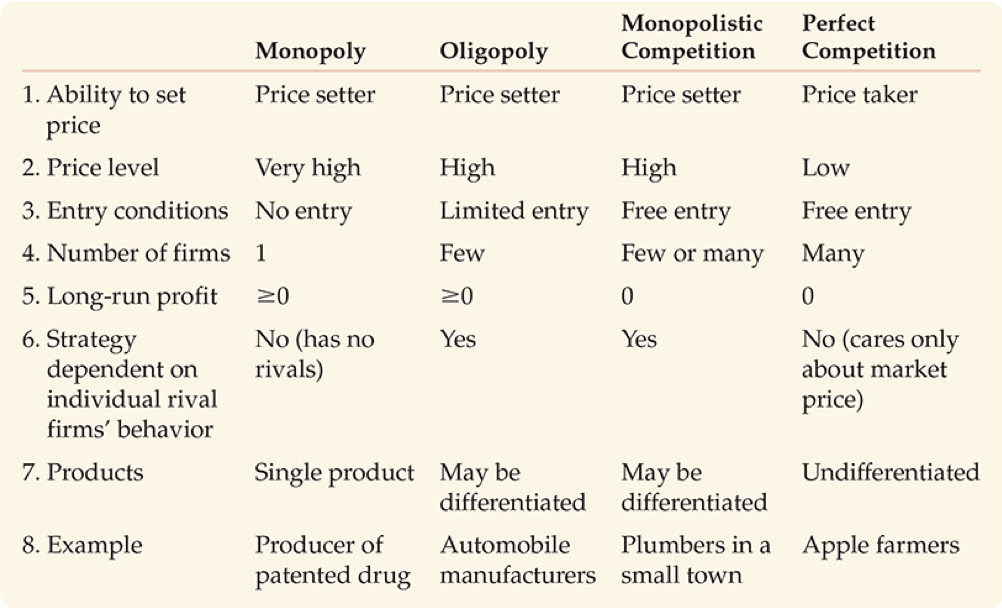
\includegraphics[scale=.65]{../images/market_structure.png}
	%\caption{A simple supply chain}
	\end{figure}
	}

\frame{
	\frametitle{Takeaways}
	\begin{enumerate}
	\item Goal of most firms: maximize profit.
		\begin{itemize}
		\item Profits are maximized when marginal revenue equals marginal cost.
		\item In some cases, it may be better to shut down than produce at all.
		\end{itemize}
	\item[]
	\item Owners and managers can have conflicting objectives.
		\begin{itemize}
		\item It is possible to create incentives to align objectives.
		\end{itemize}
	\item[]
	\item The structure of the supply chain depends on profitability of alternative forms.
	\item[]
	\item Decisions also depend on behaviour of actual and potential rivals in the market.
	\end{enumerate}
}

\end{document}
